\section{Déploiement}
\subsection{Étude de marché}
\subsubsection{Avant-propos}
Il existe de nos jours une multitude de solutions afin d'héberger une application web. Toutes les solutions offrent divers avantages et inconvénients, aussi bien d'un point de vue technologique que financier. Afin de ne pas s'encombrer avec une quantité importante de possibilités, j'ai sélectionné 3 options qui me paraissent les plus adéquates :
\begin{itemize}
  \item Serveur local
  \item Heroku (\textit{\url{https://www.heroku.com/home}})
  \item Microsoft Azure (\textit{\url{https://azure.microsoft.com/en-us/}})
  \item Virtual Private Server (VPS) chez OVH (\textit{\url{https://www.ovhcloud.com/fr/vps/}})
\end{itemize}

\newpara

Dans le cadre de ce projet, il est important de préciser les points suivant :
\begin{itemize}
  \item le client n'a \textbf{pas d'informaticien} à temps pleins
  \item le client souhaite \textbf{limiter les dépenses} au maximum
  \item le \textbf{traffic} vers l'application sera \textbf{faible} car utilisé uniquement par une ou deux personnes et pendant 2-3h par jour maximum
  \item dans le futur, un web-shop pourrait être intégré à l'application et donc générer un traffic plus important -> \textbf{évolutivité}
\end{itemize}

\newpara

La solution doit pouvoir :
\begin{itemize}
  \item Héberger une application NodeJs
  \item Héberger une base de données SQL
\end{itemize}
(Idéalement les deux services sont hébergé sur la même plateforme mais ce n'est pas obligatoire.)

\newpage
\subsubsection{Étude des solutions}
\subsubsubsection{Serveur Local} 

\textbf{Déscription}: \\ Le client utilise actuellement un serveur tournant sous Windows 10 pro. Ce serveur fait tourner leur programme de gestion mais sert également d'ordinateur "classique" pour tous les employés. Notons qu'aucun système de backup automatique n'est mis en place. La base de données inclue dans leur programme de gestion devant être accessible depuis le site de la carrosserie, une règle de port-forwarding est mise en place dans le firewall de leur routeur.

\newpara
\textbf{Avantages}:
\begin{itemize}
  \item Coût négligeable car infrastructure existante
  \item Maîtrise totale des données
\end{itemize}

\newpara
\textbf{Inconvénients}:
\begin{itemize}
  \item Os du serveur inadapté (Windows 10 pro)
  \item Maintenance plus compliqué à mettre en place
  \item Scalability (évolutivité) compliquée voir impossible sans investissement conséquent
  \item Déploiement continue plus complexe à mettre en place
  \item Accessibilité extérieur require plus de sécurité
  \item Nécessite la mise en place d'une meilleur gestion des backups
  \item Pas de redondance
\end{itemize}

\newpara
\textbf{Prix}: \\ L'infrastructure physique déjà existante et l'utilisation de software gratuit et open-source tel qu'Apache, PostgreSql, fail2ban,... rendraient les coûts négligeables.

\newpara
\textbf{Coût estimé en production}: ±0 €/mois

\newpara
\textbf{Conclusion} \\ Au vu des nombreux désavantages, je pense que cette solution, bien que peu coûteuse, ne soit pas envisageable.

\newpage
\subsubsubsection{Heroku}

\textbf{Déscription}: \\ Heroku est un PaaS(Platform as a Service) fortement utilisé de par sa simplicité et sa compatibilité avec des languages modernes tel que Node, Ruby, Python et bien d'autres.
\newpara
Bien que souvent utilisé pour des projets de petite à moyenne taille, certaines grandes entreprises comme Toyota Europe ou Dubsmash l'utilisent également.

\newpara
\textbf{Avantages}:
\begin{itemize}
  \item Intégration très facile avec git
  \item Entièrement gratuite pour le développement
  \item Inclus une base de données PostgreSql
  \item Coût en production fixe
  \item Maintenance facile et accessible à distance
  \item Portabilité élevée: il est très facile d'arrêter le service de de migré vers une autre solution. Le code n'est pas lié à Heroku
  \item Expérience: j'ai déjà plusieurs fois eu l'occasion de travailler avec Heroku, je connais assez bien la plateforme et la façon de travailler avec
  \item Métrics inclus
  \item Sécurité  
\end{itemize}

\newpara
\textbf{Inconvénients}:
\begin{itemize}
  \item Scalabilité moyenne car il faut changer de plan tarifaire en fonction du traffic
  \item Gestion de la base de données moins facile (pas de rôle différents)
  \item Cold-starts d'une à deux minutes du site-web (uniquement avec la version gratuite)
\end{itemize}

\newpara
\textbf{Prix}: \\ Heroku fonctionne sur base de plans tarifaire prédéfini mais modulable. En fonction des besoins du client, j'ai sélectionné 4 plans tarifaire:
\begin{itemize}
  \newpage
  \item \textbf{Hobby - gratuit}: \\ Ce plan tarifaire offre pratiquement toutes les fonctionnalités dont nous avons besoin. Nous serons néanmoins restraint par le nombre de requêtes, la taille de la base de données, les cold-starts, ... Cette solution me semble plus que suffisante durant le développement de l'application et pourquoi pas durant les premièrs mois ou premières années d'utilisation. Attention, la DB gratuite est limitée à 10K lignes.
  \begin{figure}[H]
    \centering
    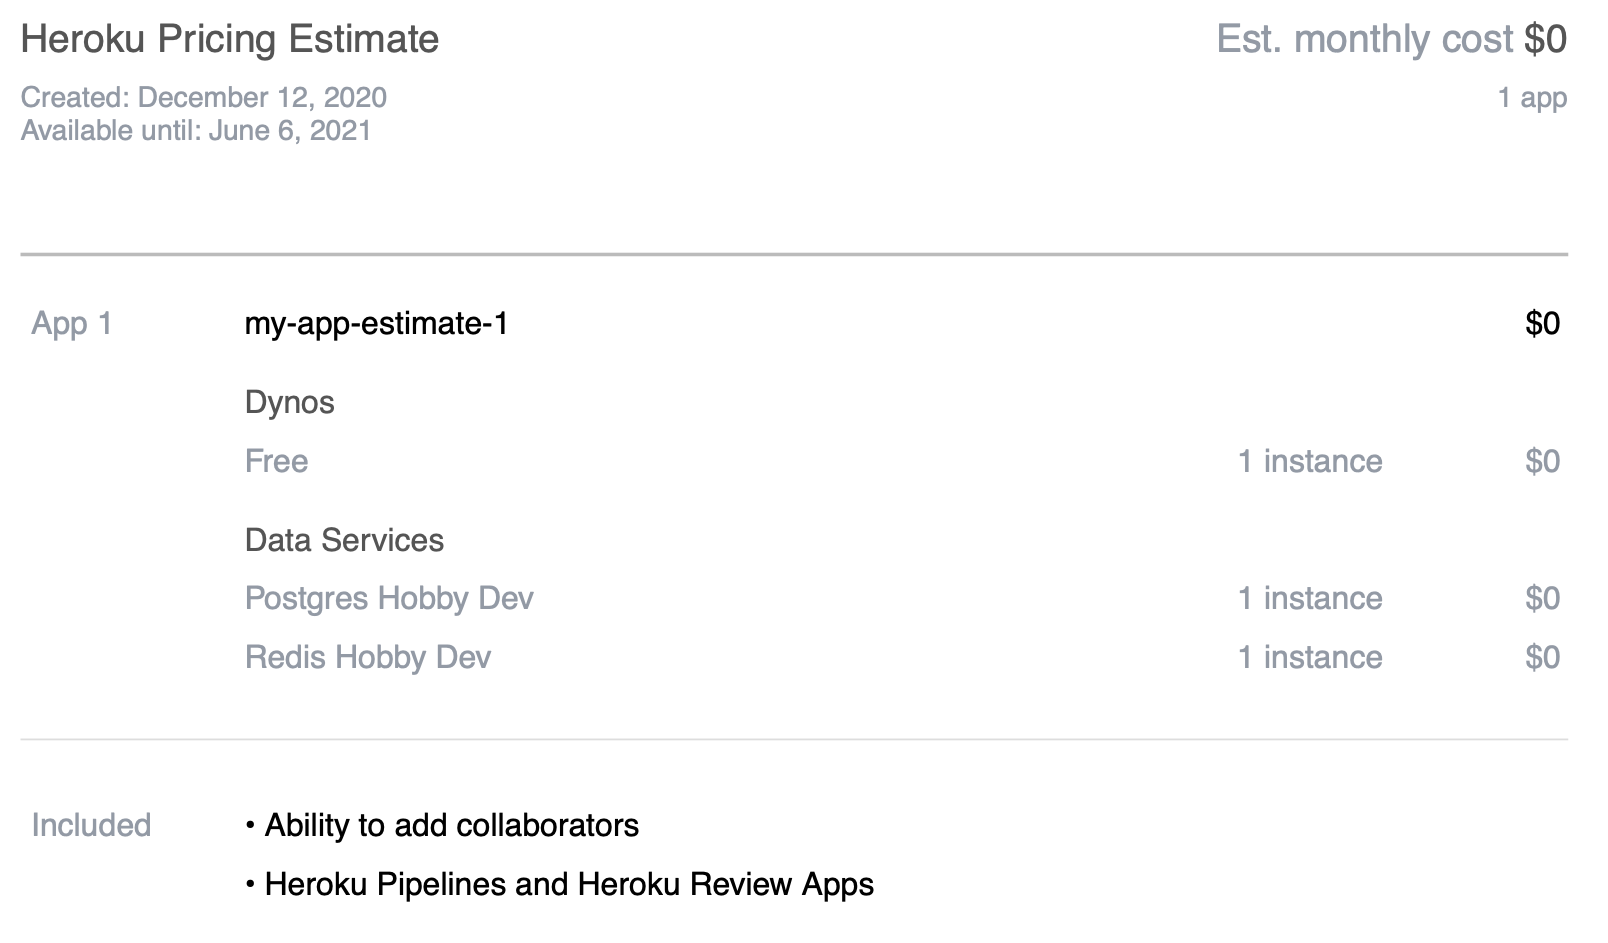
\includegraphics[width=0.75\linewidth]{img/heroku/Heroku_free.png}
  \end{figure}

  \item \textbf{Hobby - basic}: \\ Ce plan tarifaire est identique au précédent sauf que la DB peut accueillir 10M de lignes.
  \begin{figure}[H]
    \centering
    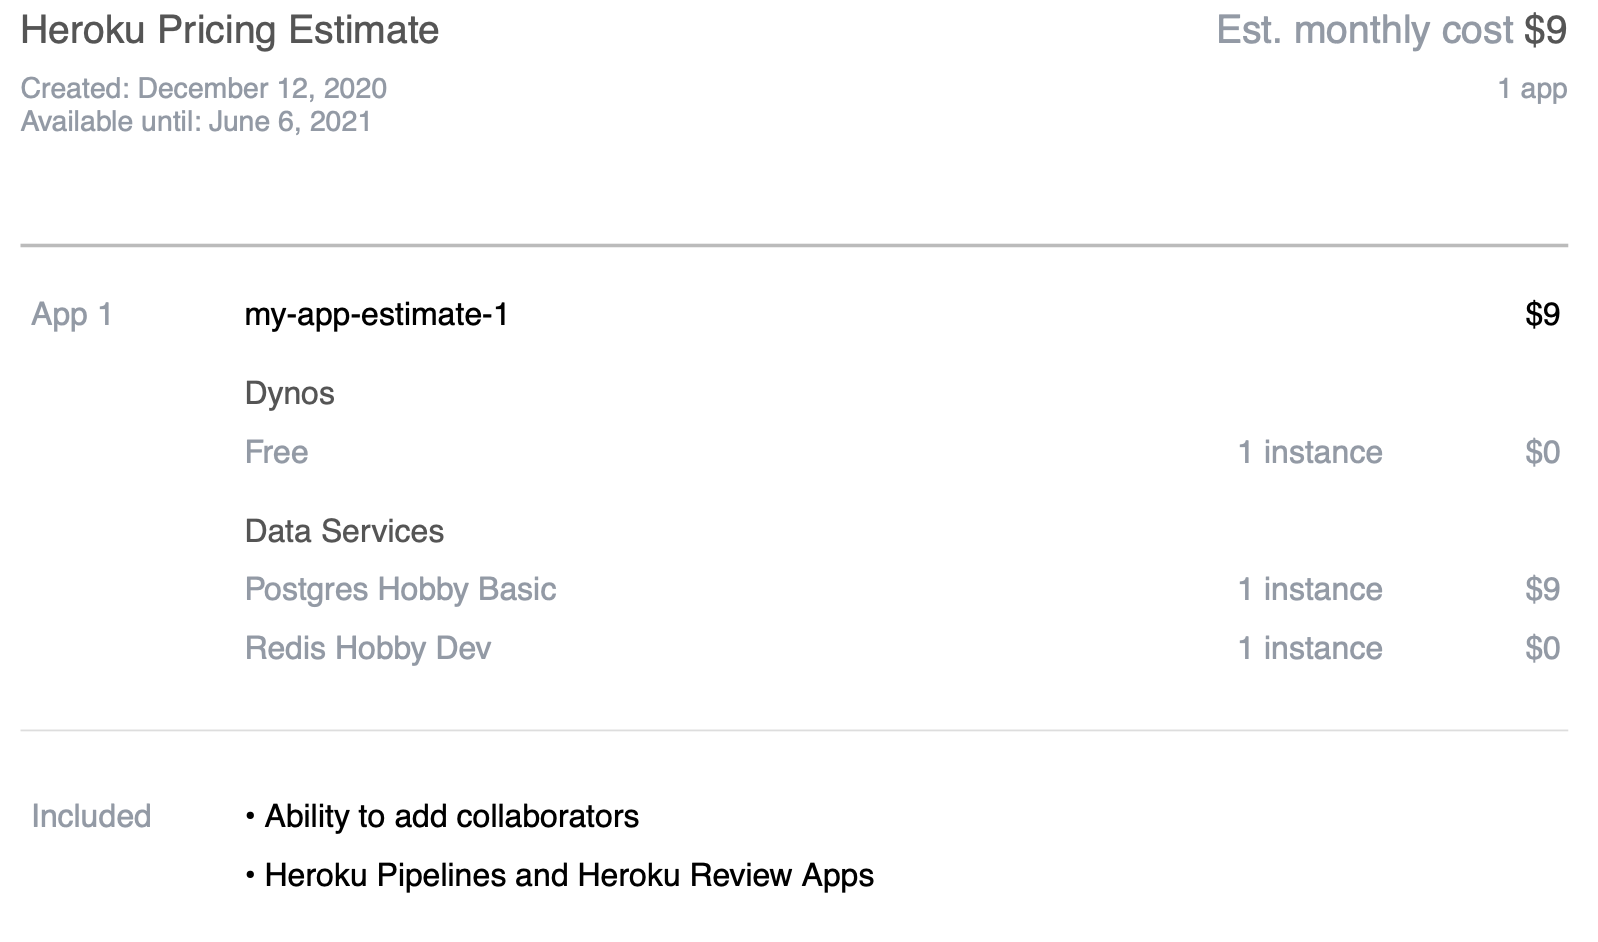
\includegraphics[width=0.75\linewidth]{img/heroku/Heroku_basic.png}
  \end{figure}
  
  \newpage
  \item \textbf{Hobby - avancé}: \\ Ce plan tarifaire est à peu de choses prêt équivalent au plan gratuit. Il permet néanmoins de supprimer complètements les cold-starts. Il offre également un les métriques du site pour les dernières 24h.
  \begin{figure}[H]
    \centering
    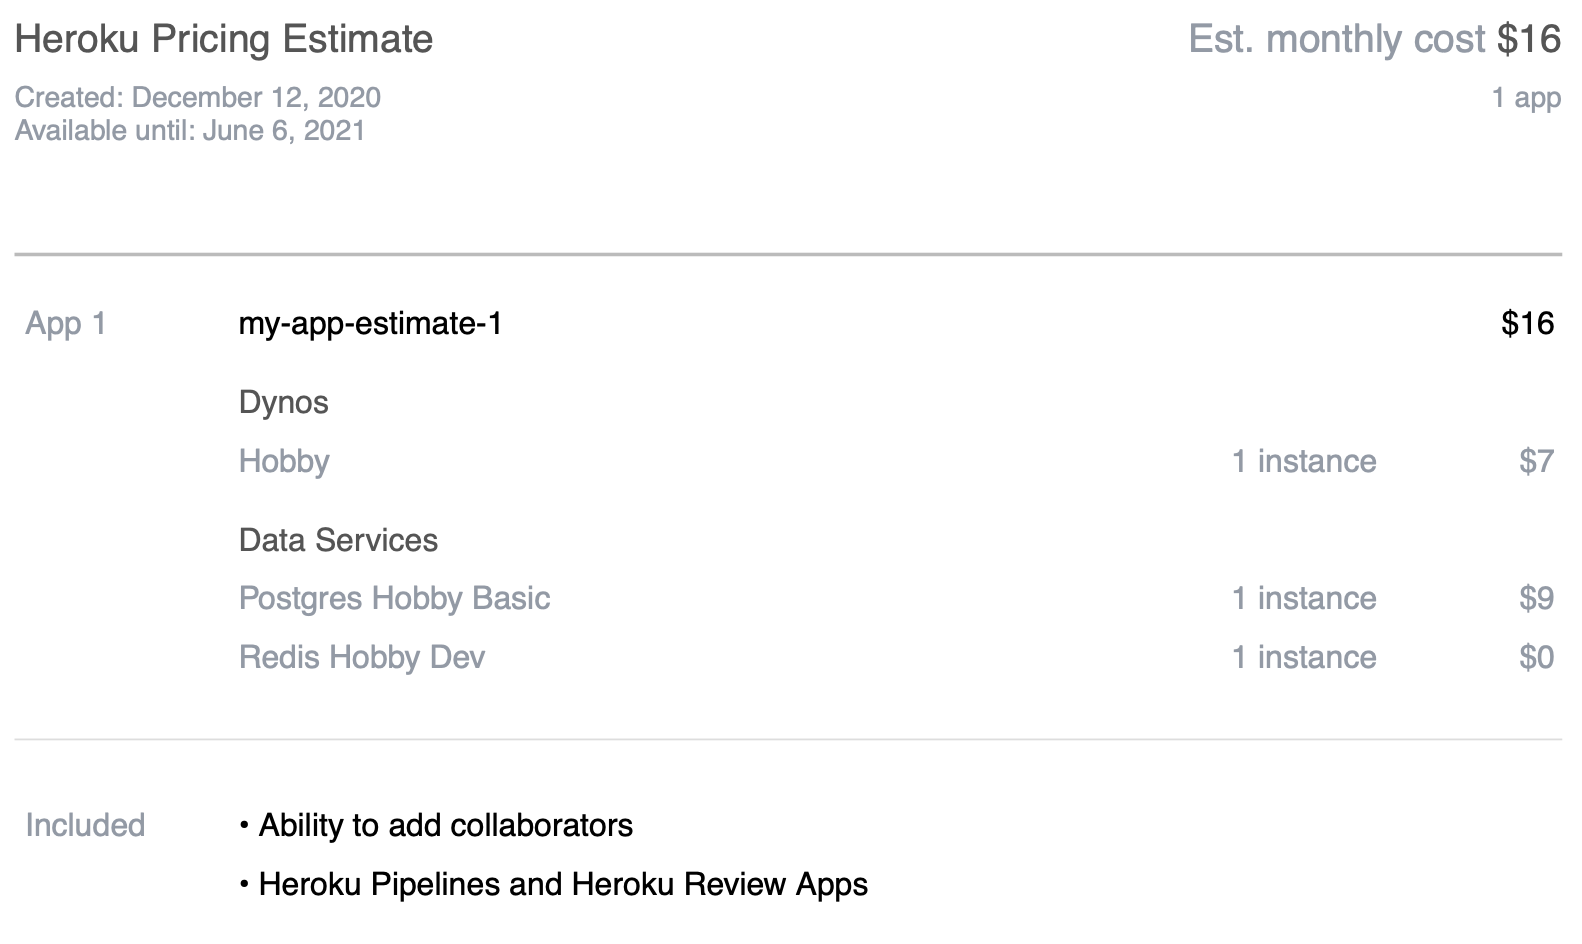
\includegraphics[width=0.75\linewidth]{img/heroku/Heroku_hobby.png}
  \end{figure}
  
  \item \textbf{Production}: \\ Cet plan offre tout ce que les plans précédents offraient mais augmente considérablement les capacité de gestion de traffic, augmente la taille maximale de la base de données, offre des métriques détaillées aussi bien pour la base de données que pour le site-web, permet des roll-backs sur une période de 7 jours.
  \begin{figure}[H]
    \centering
    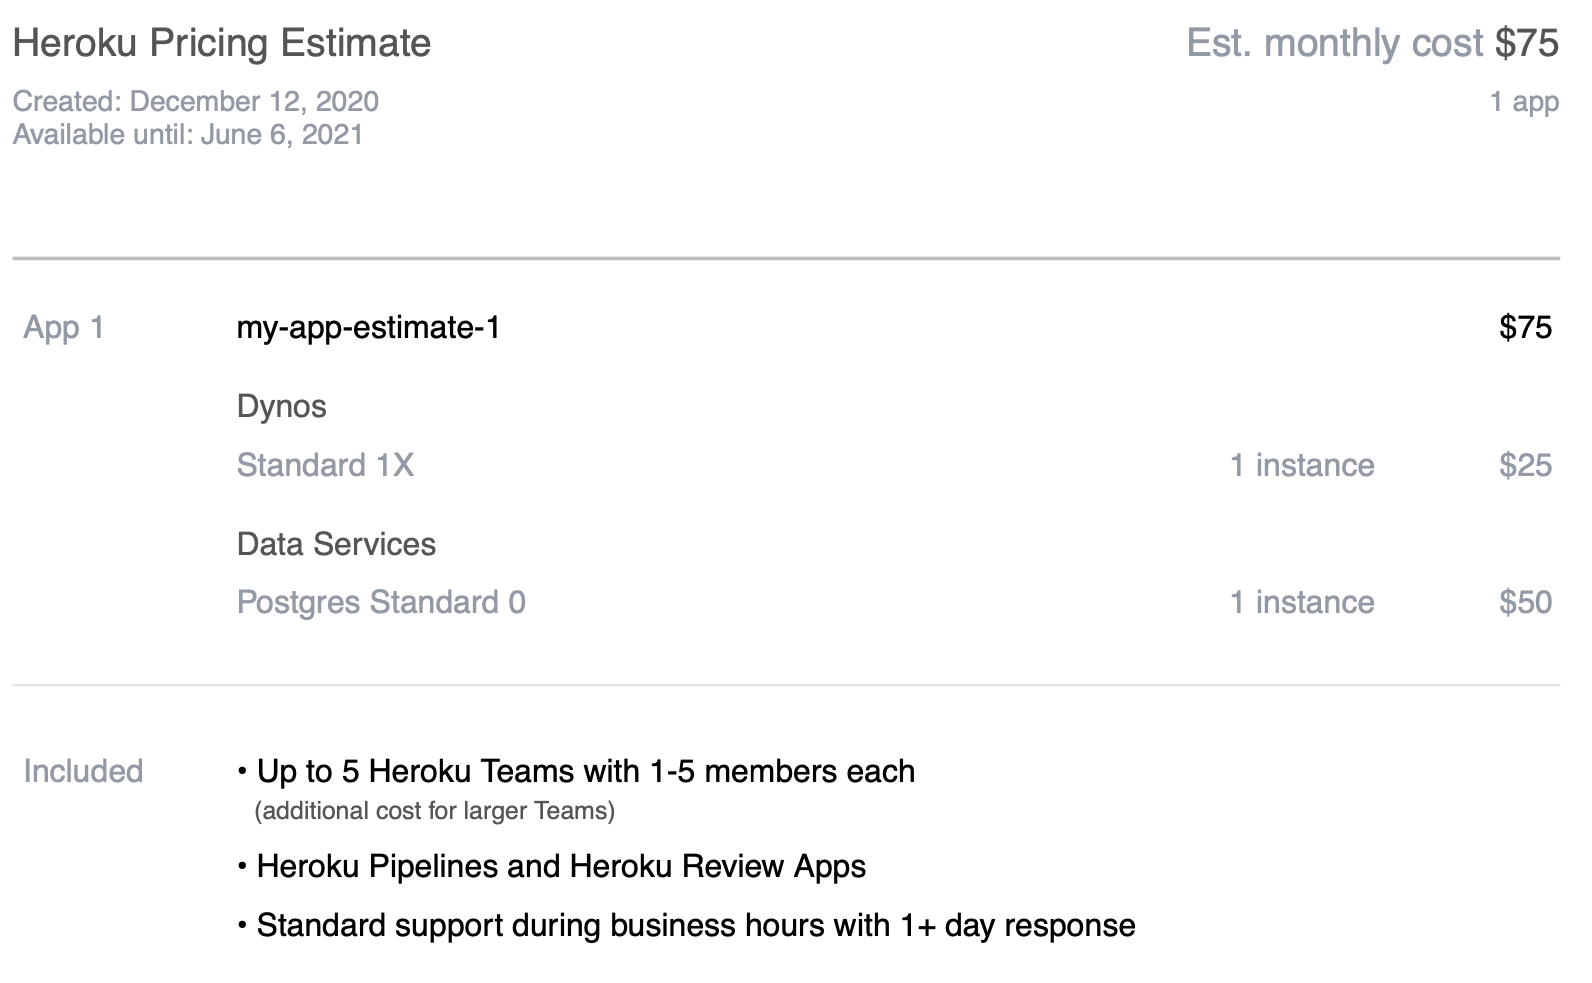
\includegraphics[width=0.75\linewidth]{img/heroku/Heroku_prod.png}
  \end{figure}
\end{itemize}

\newpage
\textbf{Conclusion} \\ Sur base de ces options, je pense qu'il est possible de partir dans un premier temps sur le plan tarifaire n°2. Néanmoins le jour où un web-shop est ajouté à l'application, il faudra probablement passer sur un autre plan tarifaire tel que le n°3.
\newpara
En plus du coût du plan n°2, il est bon de prendre une petite marge de sécurité afin de ne pas être surpris lors d'éventuels coûts supplémentaires tel qu'un nom de domaine, un autre certificat SSL,...

\newpara
\textbf{Coût estimé en production}: 18 €/mois

\newpage
\subsubsubsection{Microsoft Azure}

\textbf{Déscription}: \\ Microsoft Azure est un des leaders dans le domaine des cloud service providers. La plateforme offre plus de 200 produits couvrant une multitudes de domaines allant de la location de resources de calculs pour du Machine Learaning à l'hébergement de base de données en passant par la gestions de conteneurs Docker.
\newpara
Microsoft Azure est utilisé par un très grands nombre d'entreprises tel que 3M, Airbus, Avid, BMW et bien d'autres.

\newpara
\textbf{Avantages}:
\begin{itemize}
  \item Scalabilité extrêmement performante
  \item Compartimentation de chaque service
  \item Documentation et communauté très active
  \item Grandes flexibilité de configuration
  \item Maintenance facile et accessible à distance
  \item Métrics inclus
  \item Sécurité
\end{itemize}

\newpara
\textbf{Inconvénients}:
\begin{itemize}
  \item Coût très variable et difficile à prévoir à l'avance
  \item Complexe à configurer correctement
  \item Plus de choses à configurer manuellement
  \item Je n'ai aucune expérience
\end{itemize}

\newpara
\textbf{Prix}: \\ A l'inverse de Heroku, Azure ne fonctionne pas sur base de plans tarifaire spécifique mais fonctionne sur base du principe Pay-as-you-go. Le coût dépend donc fortement du traffic, de la taille de la base de données, de la taille des requêtes etc.

\begin{itemize}
  \item \textbf{Service Web}: Hébergement de l'app sur une machine Linux :
  \begin{itemize}
    \item version gratuite pendant 12 mois
    \item version payante : 11.081€/mois
  \end{itemize}
  \item \textbf{Base de donnée}:
  \begin{itemize}
    \item 5GB (5GB étant le minimum configurable) d'espace de stockage à 0.1155€/GB/mois soit : ±5.8€/mois
    \item 1 vCore à 0.4840€/heure, si utilisation 2h/j -> 60h/mois soit : ±29€/mois
  \end{itemize}
\end{itemize}

\newpara
\textbf{Coût estimé en production}: 50 €/mois

\newpara
\textbf{Conclusion} \\ Bien que Microsoft Azure offre une très grande flexibilité et environnement très professionnel, le coût semble fort élevé et pas très compétitif pour une application de cette envergure. Néanmoins, le jour où un web-store est ajouté, cette solution peut être retenue!

\newpage
\subsubsubsection{VPS OVH}

\textbf{Déscription}: \\ Un VPS est une machine virtuelle louée en tant que service. 

\newpara
\textbf{Avantages}:
\begin{itemize}
  \item 
\end{itemize}

\newpara
\textbf{Inconvénients}:
\begin{itemize}
  \item 
\end{itemize}

\newpara
\textbf{Prix}:

\newpara
\textbf{Coût estimé en production}: ±0 €/mois

\subsection{Première approche - Heroku}
\subsection{Seconde approche - VPS}
\subsubsection{Scirpts}
\subsubsection{Dockerisation}
\subsubsection{Sécurité}
\subsubsubsection{SSH}
\subsubsubsection{Fail2ban}
\subsubsubsection{Firewall (UFW)}
\subsubsubsection{Firewall (OVH)}


\subsection{Déploiement Continu}